% This LaTeX was auto-generated from MATLAB code.
% To make changes, update the MATLAB code and export to LaTeX again.

\documentclass{article}
\usepackage[english, russian]{babel}
\usepackage[utf8]{inputenc}
\usepackage[T1]{fontenc}
\usepackage{lmodern}
\usepackage{graphicx}
\usepackage{color}
\usepackage{listings}
\usepackage{hyperref}
\usepackage{amsmath}
\usepackage{amsfonts}
\usepackage{epstopdf}
\usepackage{matlab}

\sloppy
\epstopdfsetup{outdir=./}
\graphicspath{ {./ga_images/} }

\begin{document}

\begin{par}
\begin{flushleft}
1 Декодирование DTMF сигнала с помощью алгоритма Герцеля
\end{flushleft}
\end{par}

\begin{par}
\begin{flushleft}
1.1 Инициализация и формирование значений основных параметров
\end{flushleft}
\end{par}

\begin{matlabcode}
clear all; % Очистка памяти
close all; % Закрытие всех окон с графиками
clc; % Очистка окна команд и сообщений
fontSize = 10; % Размер шрифта графиков
tColor = 'b'; % Цвет графиков во временной области
fColor = [1 0.4 0]; % Цвет графиков в частотной области
DTMFfreqs = [697 770 852 941 1209 1336 1477 1633]; % Тоновый набор DTMF
\end{matlabcode}


\begin{par}
\begin{flushleft}
1.2 Запись аудиосигнала с микрофона
\end{flushleft}
\end{par}

\begin{matlabcode}
Fs=8000; % Частота дискретизации аудиозаписи
Nseconds = 2; % Время записи сигнала
% Запись сигнала с микрофона
recorder = audiorecorder(Fs,16,1);
recordblocking(recorder,Nseconds);
% Чтение отсчётов аудиосигнала в массив
x = getaudiodata(recorder,'uint8');
% Запись звукового файла с записанным сигналом
audiowrite('DTMF\record.wav',x(Fs/2-1:end),Fs);
\end{matlabcode}


\begin{par}
\begin{flushleft}
1.3 Чтение аудиосигнала для декодирования
\end{flushleft}
\end{par}

\begin{matlabcode}
[data,rate] = audioread('DTMF\6.wav'); % 0..9, A..D, star, sharp или record.wav
t = linspace(0, length(data)/rate, length(data)); % Формирование области определения
figure; plot(t, data, 'Color', tColor);
set(get(gcf, 'CurrentAxes'), 'FontSize', fontSize); % Изменение шрифта
title('\rm Декодируемый сигнал во временной области'); % Заголовок
xlabel('Время,\it nT_д\rm, с'); % Надпись оси абсцисс
ylabel('Сигнал,\it x(nT_д )\rm, В'); % Надпись оси ординат
\end{matlabcode}
\begin{center}
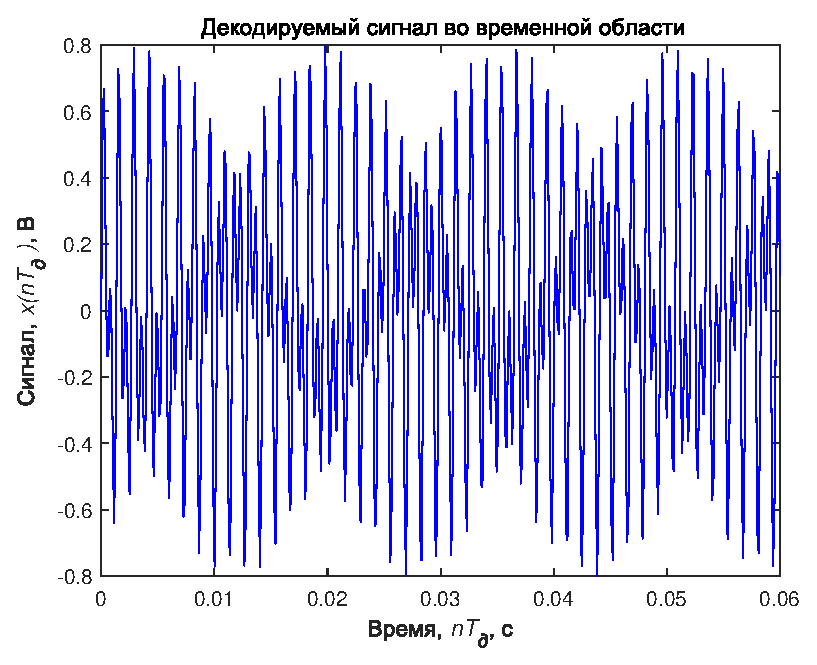
\includegraphics[width=\maxwidth{56.196688409433015em}]{figure_0}
\end{center}


\begin{par}
\begin{flushleft}
1.4 Построение амплитудного спектра декодируемого сигнала
\end{flushleft}
\end{par}

\begin{matlabcode}
f = linspace(0, rate, length(data)); % Формирование области определения
fdata = abs(fft(data)/length(data)); % Формирование значений спектра
figure; plot([-fliplr(f(1:end/2)) f(1:end/2)], fftshift(fdata),...
    'Color', fColor, 'LineWidth', 3);
xlim([-2000 2000]); % Ограничение области определения
set(get(gcf, 'CurrentAxes'), 'FontSize', fontSize); % Изменение шрифта
title('\rm Декодируемый сигнал в частотной области'); % Заголовок
xlabel('Частота,\it f\rm, Гц'); % Надпись оси абсцисс
ylabel('Амплитуда,\it A(f)\rm, В'); % Надпись оси ординат
\end{matlabcode}
\begin{center}
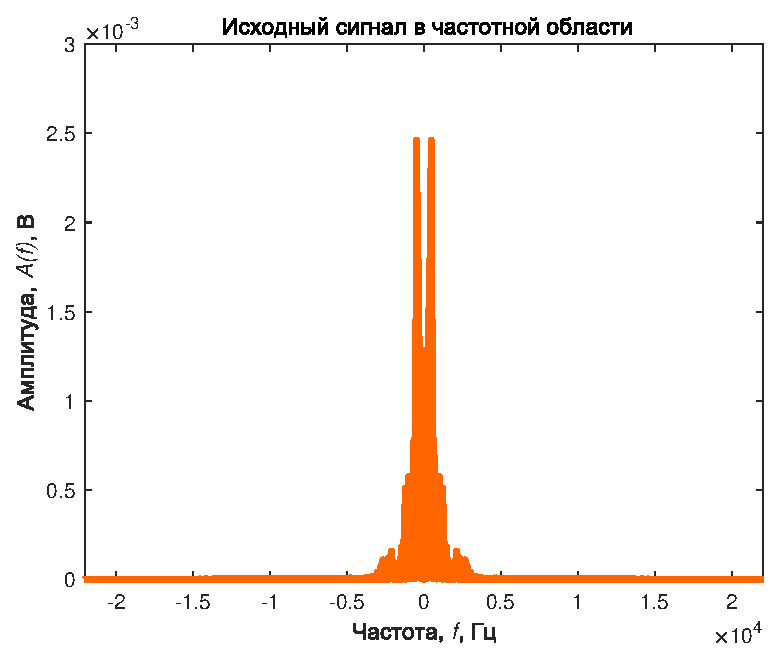
\includegraphics[width=\maxwidth{56.196688409433015em}]{figure_1}
\end{center}


\begin{par}
\begin{flushleft}
1.5 Построение амплитудного спектра в области тонового набора DTMF
\end{flushleft}
\end{par}

\begin{matlabcode}
figure; plot([-fliplr(f(1:end/2)) f(1:end/2)], fftshift(fdata),...
    'Color', fColor, 'LineWidth', 3);
xlim([600 1700]); % Ограничение области определения тоновым набором
xticks(DTMFfreqs); % Подписать только частоты из тонового набора DTMF
set(get(gcf, 'CurrentAxes'), 'FontSize', fontSize); % Изменение шрифта
title('\rm Декодируемый сигнал в частотной области'); % Заголовок
xlabel('Частота,\it f\rm, Гц'); % Надпись оси абсцисс
ylabel('Амплитуда,\it A(f)\rm, В'); % Надпись оси ординат
\end{matlabcode}
\begin{center}
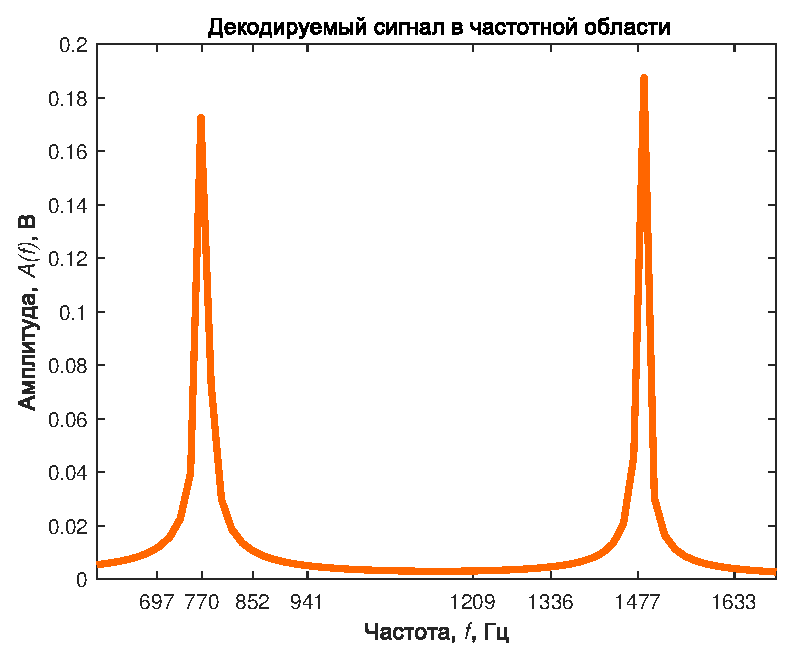
\includegraphics[width=\maxwidth{56.196688409433015em}]{figure_2}
\end{center}


\begin{par}
\begin{flushleft}
1.6 Построение дискретного амплитудного спектра с помощью алгоритма Герцеля
\end{flushleft}
\end{par}

\begin{matlabcode}
N = 205; % Количество точек ДПФ
% Расчёт номеров спектральных отсчётов для тонового набора
freq_indexes = round(DTMFfreqs/rate*N) + 1;   
% Вычисление значений спектра по алгоритму Герцеля
gdata = abs(goertzel(data(1:N),freq_indexes))/N;
% Построение графика полученного спектра
stem(DTMFfreqs, gdata, 'Color', fColor, 'LineWidth', 2);
ax = gca; % Получение текущей системы координат
ax.XTick = DTMFfreqs; % Подпись делений оси абсцисс
set(get(gcf, 'CurrentAxes'), 'FontSize', fontSize); % Изменение шрифта
title('\rm Дискретный спектр декодируемого сигнала'); % Заголовок
xlabel('Частота,\it f\rm, Гц'); % Надпись оси абсцисс
ylabel('Амплитуда,\it A(f)\rm, В'); % Надпись оси ординат
\end{matlabcode}
\begin{center}
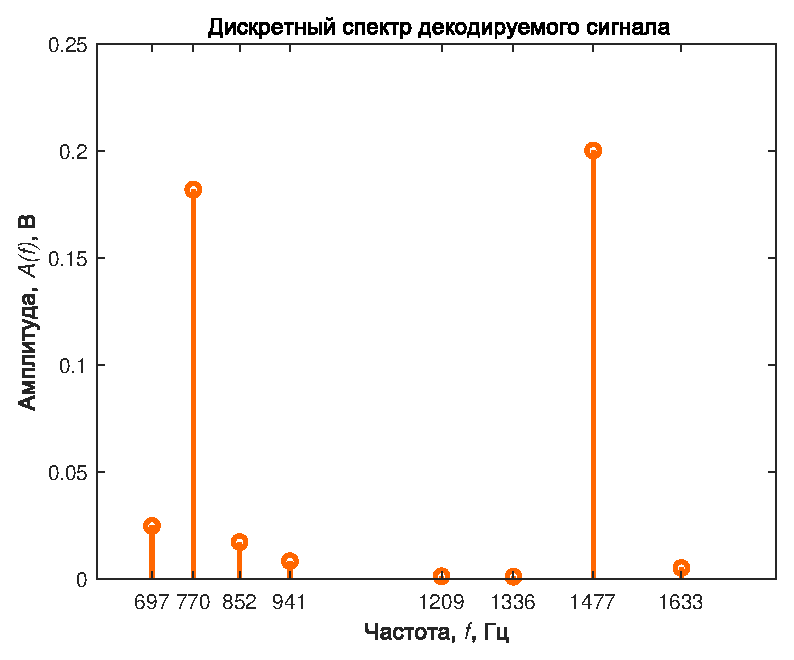
\includegraphics[width=\maxwidth{56.196688409433015em}]{figure_3}
\end{center}


\begin{par}
\begin{flushleft}
1.7 Декодирование сигнала по рассчитанным значениям спектра
\end{flushleft}
\end{par}

\begin{matlabcode}
% Матрица символов DTMF
DTMF_symbols = ['1' '2' '3' 'A';
                '4' '5' '6' 'B';
                '7' '8' '9' 'C';
                '*' '0' '#' 'D'];
% Нахождение двух наибольших частот
[value, row] = max(gdata(1:4));
[value, column] = max(gdata(5:8));
% Вывод декодированного символа
fprintf('Распознанный символ: %s\n', DTMF_symbols(row,column));
\end{matlabcode}
\begin{matlaboutput}
Распознанный символ: 6
\end{matlaboutput}

\end{document}
